\documentclass[a4paper,10pt]{article}
\usepackage[utf8]{inputenc}
\usepackage[slovene]{babel}
\usepackage[left=2cm,top=2.3cm,right=2cm,nohead]{geometry}
\usepackage{amsmath}
\usepackage{amsfonts}
\usepackage{amssymb}
\usepackage[pdftex]{graphicx}
\usepackage{subfig}
\usepackage{textcomp}
\usepackage{tikz}
\usepackage{hyperref}

\usetikzlibrary{positioning,shapes,shadows,arrows,calc,through,backgrounds}

\def\sectionautorefname{poglavje}
\def\subsectionautorefname{podpoglavje}

\hypersetup{pdfborder=0 0 0}

\begin{document}
\begin{titlepage}
  \let\footnotesize\small
  \let\footnoterule\relax
  \let \footnote \thanks
  \null\vfil
  \vskip 60pt
  \begin{center}
    {\LARGE \textbf{Hivemind} \\ Porazdeljeni Quake 2 bot \par}
    \vskip 3em
    {\large
     \lineskip .75em
      \begin{tabular}[t]{c}
        Grega Kešpret \\
        Jernej Kos \\
        Anže Vavpetič
      \end{tabular}\par}
      \vskip 1.5em
    {\large \today \par}
  \end{center}\par
  \vfil\null
\end{titlepage}

\tableofcontents
\pagebreak

\section{Predstavitev in razdelitev problema}

Cilj naše seminarske naloge je bil izdelava skupine avtonomnih botov (agentov), ki so zmožni navigacije po navideznem svetu ter medsebojne komunikacije. Navidezni svet smo si izbrali zaradi lažje izdelave senzorjev, saj se nam pri tem ni bilo potrebno ukvarjati s težavami računalniškega vida, ki sam po sebi predstavlja široko področje.

Da bi se torej izognili tem težavam, smo si za navidezno okolje v katerem bodo agenti delovali izbrali svet Quake II. Razlog za to izbiro je, da je implementacija tega sveta že na voljo in sicer pod odprtokodno licenco. To omogoča boljše razumevanje delovanja in tudi morebitne popravke ter integracijo.

Problem smo razdelili na nekaj ključnih podproblemov, katere je potrebno rešiti, da bo avtonomni agent v takem okolju deloval zadovljivo:
\begin{enumerate}
  \item \textbf{Vmesnik do navideznega sveta} je prvi korak, ki omogoča našemu agentu interakcijo z objekti v svetu in tudi povratno informacijo o rezultatih njegovih akcij.
  
  \item \textbf{Nadzor gibanja} je najnižja komponenta sistema, ki omogoča da se agent premika po svetu. Zadovoljiv nadzor gibanja mora omogočati \textit{reaktivno in samodejno izogibanje oviram} transparentno glede na to kaj zahtevajo višji nivoji. Sem spadajo tudi osnovni senzorji potrebni za pridobitev informacij o geometriji sveta.
  
  \item \textbf{Navigacija po svetu} omogoča agentu, da si zgradi notranjo predstavitev virtualnega sveta okoli njega, ki mu omogoča učinkovito načrtovanje poti v njem.
  
  \item \textbf{Stanja agenta} določajo trenutno obnašanje in cilje agenta na najvišjem nivoju.
  
  \item \textbf{Komunikacija} omogoča da se večje število agentov poveže v skupino, katere člani si lahko izmenjujejo znanje o svetu in ga tako hitreje spoznajo. Komunikacija omogoča tudi sodelovanje med člani skupine ter identifikacijo pripadnosti (nekakšen IFF\footnote{Identification Friend or Foe}) v primeru napadov.
\end{enumerate}

Tekom raziskovanja smo zgradili relativno preprosto ogrodje, ki omogoča implementacijo zgoraj omenjenih delov takšnega sistema. V nadaljevanju bomo najprej predstavili hiter pregled arhitekture ter potem lastnosti vsake komponente. Med razvojem so se nekatere prvotno zamišljene rešitve izkazale kot slabe in primorani smo jih bili zamenjati. Tudi te smo dokumentirali in opisali njihove pomanjkljivosti.

\section{Pregled arhitekture rešitve}

% Shema arhitekture
\begin{center}
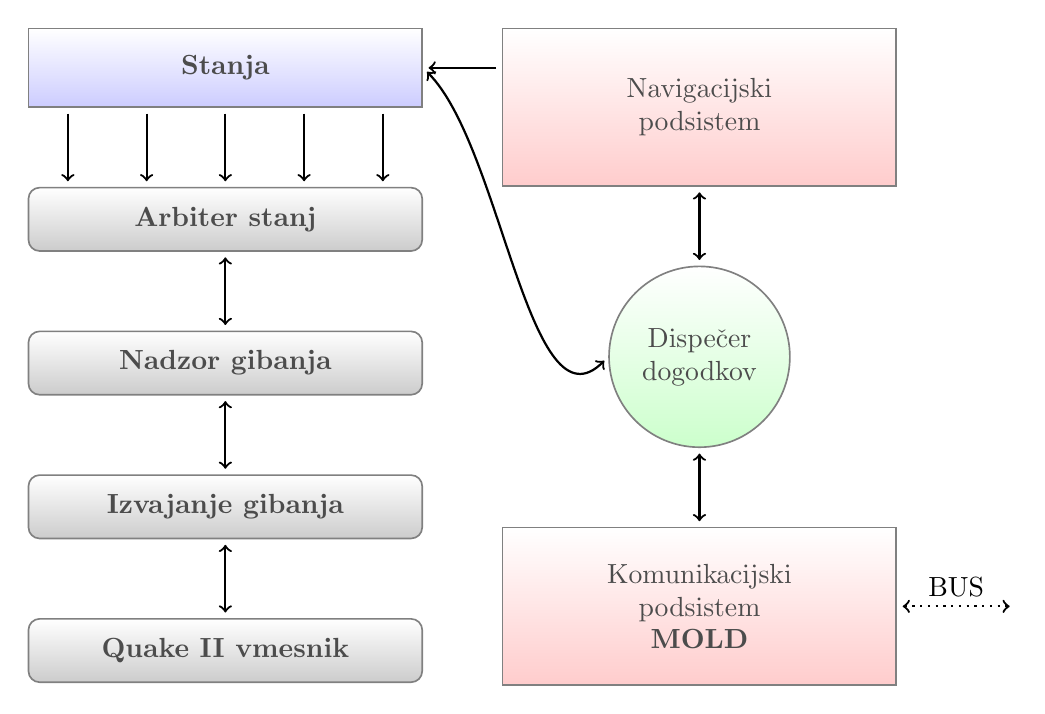
\begin{tikzpicture}[
  semithick,
	node distance=10mm,
	every node/.style={
		text centered
	},
	every path/.style={
		shorten >=2pt,
		shorten <=2pt,
		thick,
		arrows=-stealth'
	},
	colorednode/.style={
		color=black!70,
		rectangle,
		minimum height=6mm,
		minimum width=5cm,
		semithick,
		draw=black!50,
		top color=white,
		bottom color=black!20,
		rounded corners,
		inner sep=7pt
	},
	states/.style={
	  color=black!70,
		rectangle,
		minimum height=1cm,
		minimum width=5cm,
		semithick,
		draw=black!50,
		top color=white,
		bottom color=blue!20,
		inner sep=7pt
	},
	subsystem/.style={
	  color=black!70,
		rectangle,
		minimum height=2cm,
		minimum width=5cm,
		semithick,
		draw=black!50,
		top color=white,
		bottom color=red!20,
		inner sep=7pt
	},
	dispatcher/.style={
	  color=black!70,
		circle,
		minimum height=2cm,
		minimum width=2cm,
		semithick,
		draw=black!50,
		top color=white,
		bottom color=green!20,
		inner sep=7pt
	}
]

  \node (Q2Vmesnik) [colorednode] { \textbf{Quake II vmesnik} };
  \node (IzvajanjeGibanja) [colorednode, above=of Q2Vmesnik] { \textbf{Izvajanje gibanja} };
  \node (NadzorGibanja) [colorednode, above=of IzvajanjeGibanja] { \textbf{Nadzor gibanja} };
  \node (Arbiter) [colorednode, above=of NadzorGibanja] { \textbf{Arbiter stanj} };
  \node (Stanja) [states, above=of Arbiter] { \textbf{Stanja} };
  \node (Navigacija) [subsystem, right=of Stanja, yshift=-5mm] { \shortstack{ Navigacijski \\ podsistem } };
  \node (Dispatcher) [dispatcher, below=of Navigacija] { \shortstack{ Dispečer \\ dogodkov } };
  \node (Komunikacija) [subsystem, below=of Dispatcher] { \shortstack{ Komunikacijski \\ podsistem \\ \textbf{ MOLD } } };
  
  \draw[->] ($ (Stanja.south) - (2cm,0) $) -- ($ (Arbiter.north) - (2cm,0) $);
  \draw[->] ($ (Stanja.south) - (1cm,0) $) -- ($ (Arbiter.north) - (1cm,0) $);
  \draw[->] ($ (Stanja.south) - (0cm,0) $) -- ($ (Arbiter.north) - (0cm,0) $);
  \draw[->] ($ (Stanja.south) + (1cm,0) $) -- ($ (Arbiter.north) + (1cm,0) $);
  \draw[->] ($ (Stanja.south) + (2cm,0) $) -- ($ (Arbiter.north) + (2cm,0) $);
  \draw[<->] (Arbiter) -- (NadzorGibanja);
  \draw[<->] (NadzorGibanja) -- (IzvajanjeGibanja);
  \draw[<->] (IzvajanjeGibanja) -- (Q2Vmesnik);
  
  \draw[->] ($ (Navigacija.west) + (0,5mm) $) -- (Stanja);
  \draw[<->] (Navigacija) -- (Dispatcher);
  \draw[<->] (Dispatcher) -- (Komunikacija);
  \draw[<->] (Stanja.east) .. controls +(1,-1) and +(-1,-1) .. (Dispatcher.west);
  
  \draw[<->,dotted] (Komunikacija.east) -- node[above] {BUS} +(1.5cm,0); 
\end{tikzpicture}
\end{center}



Osnovna arhitektura močno sledi podproblemom, ki smo jih predstavili v uvodu. Posamezne komponente so organizirane kot C++ razredi, povezani preko neposrednih klicev ali pa preko dogodkov.

Celoten sistem je predstavljen s pomočjo centralne komponente imenovane \texttt{Context}. Ta komponenta povezuje vse ostale v celoto in skrbi za uspešno inicializacijo vmesnika do virtualnega sveta, komunikacijskega podsistema, dispečerja dogodkov ipd. Omogoča tudi nekaj osnovnih storitev kot je izpis sporočil za potrebe spremljanja poteka izvajanja programa.

\section{Vmesnik do virtualnega sveta}

Kot naš virtualni svet smo vzeli svet Quake II, ki omogoča dva načina vključitve v sam svet:
\begin{enumerate}
  \item \textbf{UDP/IP povezava odjemalca} se v osnovi obnaša popolnoma enako kot uraden Quake II odjemalec, ki je namenjen večigralstvu. Za to je potrebno razumevanje in implementacija Quake II protokola.
  
  \item \textbf{Integracija v naslovni prostor igre} je v osnovni namenjena t.i. \textit{strežniškim botom} pa tudi najrazličnejšim dodatkom in razširitev igre.
\end{enumerate}

Ker je cilj narediti avtonomne agente, ki niso na nikakršen način priviligirani nad ostalimi igralci, poleg tega pa morajo biti tudi sposobni delovanja iz različnih sistemov IP\footnote{V mrežo povezanih računalnikov} je edina smiselna možnost prva. Zaradi tega je bil prvi korak razumevanje in implementacija Quake II protokola ter izdelava preprostega odjemalca zanj.

Vendar pa naše ogrodje relativno transparentno podpira tudi drugi način za potrebe pospešene simulacije. Razlogi za to so opisani v enem izmed kasnejših poglavij, ki opisuje \textit{evolucijske umetne nevronske mreže}. Čeprav samega pristopa kasneje nismo uporabili, se je podpora za takšen način simulacije ohranila.

V podrobnosti obeh implementacij se na tem mestu ne  bi spuščali, pomembno je omeniti le da na svet v obeh primerih vplivamo na enak način. V vsakem trenutku moramo svetu posredovati vektorja orientacije (v obliki Eulerjevih kotov) ter hitrosti, poleg tega pa še oznako ali naj agent strelja ali ne. V drugi smeri pa so agentu periodično posredovani podatki o bližnjih dinamičnih entitetah ter o njegovi lokaciji.

Celotno ogrodje je organizirano tako, da najprej vsem komponentam sistema posreduje najnovejše znanje o bližnjem svetu (t.i. \textit{game state}), nato pa od nadzornika gibanja zahteva nov set vektorjev, ki jih preko vmesnika posreduje v svet. Vse to se mora odvijati dovolj hitro, saj svet zahteva posodobitve v realnem času.

\section{Nadzor gibanja in izogibanje oviram}

Osnovna funkcija agenta je gibanje po svetu, saj to predstavlja bistven način interakcije s svetom. V ta namen je bilo prvotno potrebno razviti sistem, ki omogoča višjim nivojem da sporočijo želeno destinacijo v obliki \textit{lokalnih koordinat} (t.j. koordinat, ki so dosegljive brez dodatnega planiranja poti).

Tak sistem mora imeti tudi sposobnost izogibanja oviram, saj bi se v nasprotnem primeru agent zaradi geometrije sveta kaj hitro zaletel v steno ali zataknil v kakšen rob. Podoben problem predstavljajo tudi prepadi in vodne pasti v katere bi agent, ki bi slepo sledil točkam kaj hitro padel.

\subsection{Senzorji}

Navidezni senzorji omogočajo zaznavanje razdalje do ovire pod določenim kotom. Podatki o statični geometriji sveta so na voljo v t.i. BSP\footnote{\textit{Binary Space Partitioning} drevesa razdelijo prostor s hiperravninami na manjše odseke in omogočajo učinkovite poizvedbe o geometriji} drevesih za katere smo morali implementirati parser in ustrezne funkcije za izvajanje poizvedb nad njimi. Tako je v osnovi mogoče izstreliti žarek iz točke A proti točki B in ugotoviti kje na poti ga prekine statična geometrija.

Agentove senzorje smo si najprej zamislili kot nekaj (v našem primeru jih je 19 v zrazponu od -90° do +90°) usmerjenih žarkov, ki v vsakem trenutku preverjajo kje se nahaja ovira. Vsi žarki so razporejeni v neki ravnini na fiksni višini glede na položaj agenta, kotom pa je dodan naključen šum +-5°, ki zmanjšuje možnost da bi agent zgrešil kakšno oviro. Tak način sicer v osnovi deluje dobro pri zaznavanju sten in večjih ovir, odpove pa na stopnicah (agent bi v tem primeru stopnice zaznal kot steno) in prepadih (teh agent sploh ne bi zaznal).

V ta namen smo preproste senzorje razdalje nadomestili s preprosto lokalno simulacijo sprehoda v dani smeri. Definirali smo dolžino koraka in simulacija je potekala tako:
\begin{enumerate}
  \item Najprej z žarkom v dani smeri preverimo ali je na naslednjem koraku slučajno stopnica in ali jo lahko prestopimo (za to je definirana maksimalna višina stopnice, ki jo agent še lahko prestopi). V primeru da jo lahko, premaknemo simulacijo na to mesto.
  
  \item Z žarkom v dani smeri preverimo ali se na dolžini koraka nahaja ovira. V kolikor se ne, prestavimo simulacijo na to mesto.
  
  \item Preverimo ali stojimo na trdnih tleh, tako da usmerimo žarek navpično navzdol od mesta simulacije. V kolikor stojimo na tleh, prestavimo simulacijo na to mesto.
  
  \item Če smo presegli maksimalno število korakov vrnemo razdaljo, sicer nazaj na prvo točko.
\end{enumerate}

Takšni senzorji se obnesejo veliko bolje, saj lahko agent sedaj pravilno zazna tako stopnice kot tudi prepade. To sicer poveča število geometričnih poizvedb (testov z žarkom), vendar se BSP drevesa izkažejo kot učinkovita optimizacija in tako te poizvedbe ne predstavljajo velikih težav.

Sami senzorji pa so zgolj orodje, ki ga mora učinkovito uporabiti nadzorni sistem za sprejetje odločitve kam naj se dejansko premakne. V naslednjih dveh podpoglavjih bomo predstavili dva pristopa, enega manj uspešnega in enega precej uspešnega.

\subsection{Nadzorni sistem z EANN}

Najprej smo želeli nadzorni sistem implementirati s t.i. evolucijskimi umetnimi nevronskimi mrežami. Gre za koncept, kjer za učenje nevronske mreže uporabljamo genetski algoritem, ki ga vodi kriterijska funkcija. V literaturi \cite{champandard02} smo zasledili da se omenjena kombinacija dobro obnese na problemski domeni nadzornih sistemov takšnih agentov, zato smo jo poskušali uporabiti.

V našem primeru so namreč tako vhodi (razdalje do ovir s senzorjev ter prejšnji izhod mreže) kot izhodi (zahtevani popravek kota) zvezne vrednosti za kar so nevronske mreže še posebej primerne (v kolikor uporabljamo ustrezno sigmoidno odzivno funkcijo), saj ne zahtevajo diskretizacije vrednosti.

\subsubsection{Topologija nevronske mreže in genetski algoritem}
Za topologijo nevronske mreže smo izbrali znani perceptron in sicer z enim skritim nivojem petih nevronov. Genom za genetski algoritem je bil tako sestavljen kar iz uteži nevronske mreže, na začetku pa so bile te uteži postavljene naključno. Osebke za križanje pri generiranju naslednje generacije smo iz populacije izbirali tako, da je bila verjetnost izbire vsakega osebka proporcionalna njegovi ustreznosti glede na kriterijsko funkcijo (ta način izbire se sicer imenuje \textit{roulette-wheel selection}).

Ker je bila naša kriterijska funkcija (o njej malce kasneje) zastavljena tako, da je bila najvišja možna vrednost 0, vsi slabši osebki pa so bili predstavljeni z negativnimi vrednostmi, je bilo potrebno pred izbiro narediti tudi transformacijo vrednosti kriterijske funkcije tako da so vse vrednosti padle na realni interval med 0 in 10. Natančna funkcija, ki smo jo uporabili pri transformaciji se nahaja v \cite{seymour08}.

\subsubsection{Kriterijska funkcija}
Kriterijska funkcija je bila zastavljena tako, da je kaznovala različne tipe obnašanja (ti atributi so povzeti po \cite{champandard02}):
\begin{itemize}
  \item Trki z objekti so bili kaznovani.
  \item Velike spremembe smeri so bile kaznovane (še posebej v kolikor ni bilo pred agentom nobene ovire).
  \item Ohranjanje smeri je bilo nagrajeno (oz. neohranjanje smeri je bilo kaznovano).
  \item Oscilacije (zaporedni popravki najprej v eno, nato pa v drugo smer) so bile kaznovane.
\end{itemize}

Na tem mestu pa je nastopila precejšnja težava. Genetski algoritem za konvergenco potrebuje dovolj veliko populacijo in veliko število generacij. Mi smo imeli na voljo enega agenta, ki je naenkrat lahko uporabljal zgolj en genom (nevronsko mrežo). Torej je bilo potrebno posamezno nevronsko mrežo uporabljati določen čas in nato kumulativno oceniti njeno ustreznost. Skupaj z velikim številom zahtevanih generacij je to predstavljalo precejšen problem, saj na hitrost simulacije nismo morali vplivati (delovala je v realnem času).

\subsubsection{Pospešena simulacija}

Edina možnost, da bi lahko preizkusili dani algoritem in povečali možnost konvergence v doglednem času je bila da na nek način pospešimo simulacijo. Za ta namen smo našemu ogrodju dodali možnost neposredne integracije v naslovni prostor simulatorja (torej igre Quake II), kjer smo lahko hitrost delovanja prilagodili. Tako smo dosegli približno 30-kratno pospešitev simulacije.

Na žalost tudi po vsem tem naporu željenih rezultatov nismo dobili, konvergenca genetskega algoritma se je ustavila v nekem popolnoma neuporabnem naboru uteži. Razloge za to gre verjetno iskati v neprilagojenosti vrednosti parametrov kriterijske funkcije ali pa morebiti v kakšnem hrošču v implementaciji. Na žalost nismo imeli časa, da bi odkrili vzrok, tako da je to ena izmed možnosti za nadaljnje raziskave. Smo pa v tem procesu našemu ogrodju dodali funkcionalnost potrebno za pospešeno simulacijo ter za uporabo genetskih algoritmov in umetnih nevronskih mrež.

\subsection{Nadzorni sistem z mehko logiko}

Med našim raziskovanjem smo kontaktirali tudi avtorja \cite{champandard02}, \textit{Alexa J. Champandarda}, ki je potrdil problematičnost uporabe EANN in priporočal, da raje naredimo preprost nadzorni sistem z mehko logiko\footnote{Fuzzy logic}. Bistvena prednost takšnega sistema je nepotrebnost iskanja po prostoru možnih obnašanj (torej učenja), prav tako pa je zaradi njegove preprostosti tak sistem brez morebitnih skritih odvisnosti (za razliko od kriterijske funkcije genetskega algoritma, kjer je včasih težko napovedati kakšne rezultate bo imela sprememba vrednosti določenega parametra).

Mehka logika se sicer veliko uporablja tudi v robotiki \cite{grayston06}, v principu pa deluje tako, da posamezne vrednosti združimo v razrede (npr. razdalja do ovire je lahko majhna, srednja ali velika; kot do ovire je lahko majhen, srednji ali velik). Nato definiramo akcije za kombinacije takšnih razredov:

\begin{verbatim}
  ČE kot = majhen IN ovira = blizu POTEM ZAVIJ(za 15°).
\end{verbatim}

Takšna obnašanja definiramo za vse kombinacije kota in razdalje do ovire. Izračun poteka v dveh fazah in sicer najprej moramo vhodne vrednosti (kot ter razdaljo) spremeniti glede na pripadnost posameznim razredom (v našem primeru so imeli razredi trapezno obliko), nato pa izračunati izhodni kot glede na definirana obnašanja z množenjem ustreznih uteži.

Ker spremenljivke nimajo grobih mej in ker se razredi deloma prekrivajo, dobimo kot izhod neverjetno gladke odzive na ovire. Ta rešitev se je torej izkazala kot zelo preprosta in zelo efektivna. Med že prej omenjenimi senzorji smo torej izbrali tistega, ki je sporočil najmanjšo razdaljo ter njegov kot ter zaznano razdaljo uporabili kot vhod v nadzorni sistem z mehko logiko. Na izhodu smo izračunali potreben popravek smeri.

\subsection{Evaluacija rešitve}

Rešitev z mehko logiko se je izkazala kot zelo robustna, agent se je uspešno izogibal prepadom, vodnim pastem in stenam. Sistem smo testirali tako, da smo agentu preprosto "ukazali" naj hodi naprej. Zaradi vključenega sistema za izogibanje oviram je brez večjih težav hodil po svetu brez da bi kam padel ali se zaletel v kakšno steno. S tem razlogom smo to rešitev ocenili kot dobro in jo obdržali v sistemu.

\section{Navigacija po svetu} \label{sec:navigacija-po-svetu}

Vmesnik do navideznega sveta skupaj z nadzornim sistemom gibanja torej že omogoča premikanje po svetu. Vendar se agent ne zaveda kje hodi, niti ne more načrtovati poti do določenih lokacij. V ta namen ima naš sistem vgrajen podsistem za navigacijo, ki omogoča da se agent sam nauči možnih poti po svetu (tako iz svojih izkušenj kot iz opazovanja drugih entitet). Takega pristopa nismo uporabili takoj na začetku, tako da bomo ponovno najprej predstavili prvotno rešitev in razloge zakaj se ta ni obnesla, ter potem zadnjo rešitev, ki uporablja omenjeno učenje.

\subsection{Statična geometrija iz BSP dreves}

Prvotna zamisel je bila, da bi graf sveta zgradili kar iz podatkov, ki so nam na voljo s pomočjo BSP drevesa v opisu sveta. Samo BSP drevo je torej sestavljeno iz množice ploskev, ki opisujejo geometrijo (statične) okolice. Iz povezave teh ploskev (stičnih robov med njimi) je mogoče zgraditi graf povezljivosti in ga uporabiti za iskanje poti.

Takšna rešitev pa ima ključni problem in sicer to, da ne temelji na dejanskih možnih premikih agenta, temveč le opisuje geometrijske relacije med ploskvami, ki predstavljajo svet. To pomeni, da so lahko povezane lokacije, ki v resnici niso prehodne zaradi najrazličnejših vplivov v sami igri. To se da do neke mere izločiti vendar v tem primeru dobimo območja, ki niso dobro povezana, pa v resnici so prehodna.

Rešitev je slaba tudi zato, ker je vezana na opis geometrije, ki v osnovi ni namenjen takšni interpretaciji (namenjen je geometrijskim poizvedbam ter izrisu sveta v običajnih odjemalcih). Zaradi teh pomanjkljivosti smo takšno rešitev opustili.

\subsection{Samodejno učenje topografije}

Naša naslednja ideja je bila: zakaj se agent ne bi sam naučil kateri premiki po svetu so mogoči in kateri ne? Tako bi lahko bil bolje prepričan kaj se da in kaj ni mogoče. Za hitrejše učenje (in ker agent včasih nima dovolj domišljije) pa bi lahko opazoval tudi druge dinamične entitete (igralce) v lokalni okolici in se učil tudi na podlagi njihovih premikov.

Bistvo ideje je naslednje - v kolikor sem se uspešno premaknil iz točke A na točko B, obstaja velika verjetnost da sta ti dve točki povezani. Potrebno je zgolj definirati način, kako te premike učinkovito spraviti v obliko, ki je ustrezna za kasnejše preiskovanje (torej graf).

\begin{figure}[h]
 \centering
 \subfloat[Tipične poti agenta skozi svet]{\label{fig:grid-path}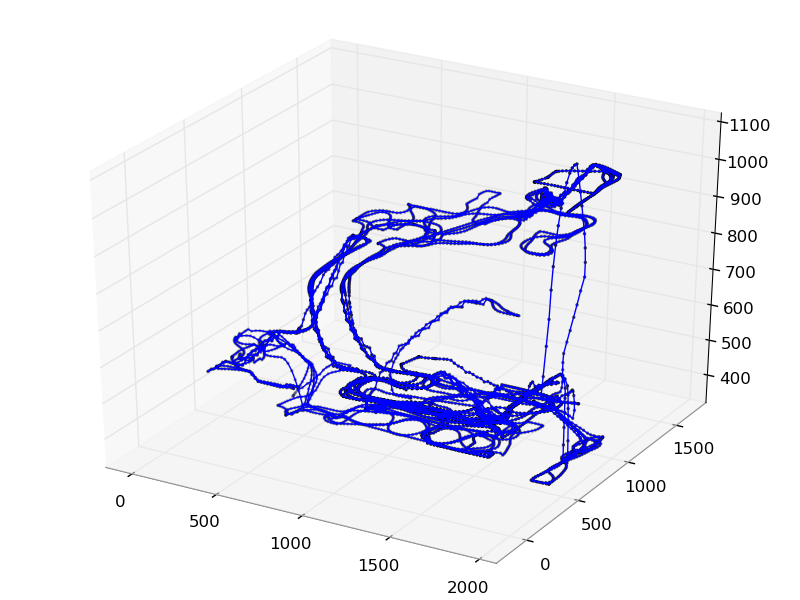
\includegraphics[width=253px]{hm-grid-path.png}}
 \subfloat[Graf zgrajen na podlagi premikov]{\label{fig:grid-graph}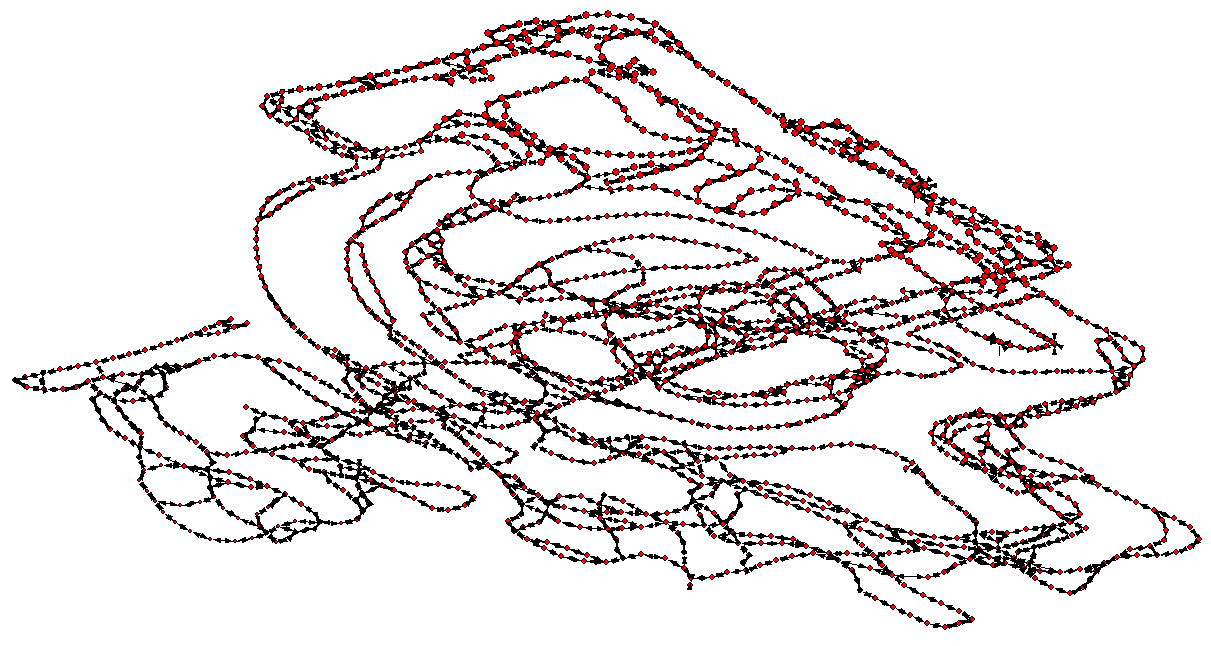
\includegraphics[width=253px]{hm-grid-graph.png}}
 \caption{Samodejno učenje topografije sveta transformira poti v kompaktnejši graf, ki je primeren za iskanje}
 \label{fig:grid}
\end{figure}

\noindent
Na sliki \ref{fig:grid-path} lahko vidimo poti agenta skozi svet. Ker se agent nikoli ne premika enako, lahko posamezne točke na isti poti precej odstopajo ena od druge. Kljub temu bi želeli da so v grafu vse te točke predstavljene zgolj kot eno vozlišče, saj v nasprotnem primeru to nepotrebno povečuje graf.

V ta namen smo uvedli dva koncepta:
\begin{enumerate}
  \item \textbf{Točke} (\textit{waypoints}) predstavljajo poljubne lokacije v prostoru, kjer se je agent lahko nahajal.
  
  \item \textbf{Vozlišča} (\textit{nodes}) predstavljajo lokacijo v grafu, ki lahko zajema večje število bližnjih točk. V kolikor vozlišča na določeni lokaciji ni, se samodejno ustvari ko obstaja prva točka na tej lokaciji. Vsako vozlišče ima svoj radij in vse točke, ki padejo v ta radij se nahajajo v istem vozlišču.
\end{enumerate}

Hitra lokalizacija posameznih vozlišč je za ta pristop ključnega pomena, zato smo uporabili podatkovno strukturo kd-drevesa (v našem primeru $k = 3$, saj je svet opisan v treh dimenzijah). Ta nam omogoča da v logaritemskem času najdemo vozlišče, ki je najbližje določenim koordinatam in s tem zmanjšanje vozlišč v grafu. V ogrodju uporabljamo C++ implementacijo kd-dreves iz \cite{harris08}.

Za boljšo vizualizacijo tako naučenega grafa smo v ogrodje dodali možnost izvoza grafa v format, ki je primeren za obdelavo v programskem paketu Pajek \cite{batagelj97}, primer izrisa je viden v sliki \ref{fig:grid-graph}.

\subsubsection{Posodabljanje topografije glede na zunanje informacije}

Naš agent ima sposobnost, da znanje o svetu dinamično prilagaja. V ta namen ima komponento, ki se odziva na dogodke o na novo odkritih entitetah in njihovih premikih. V kolikor agent nastopa v skupini, si te informacije izmenjuje tudi z drugimi agenti znotraj skupine. Vsako točko, ki jo na tak način vidi oz. zazna, takoj doda v notranjo predstavitev sveta, kljub temu da mogoče še ni dosegljiva. Takoj ko kasneje opazi povezavo med takšno točko (ali celo nepovezano komponento grafa) in preostalim delom sveta jo poveže, tako da so vse informacije nemudoma na voljo.

To izboljša hitrost grajenja predstave o svetu, saj omogoča da se topografija gradi vzporedno glede na znanje celotne skupine oz. drugih entitet, ki so morda vidne, vendar se nahajajo zunaj znanega grafa.

\subsection{Iskanje poti skozi svet}

Ko imamo graf enkrat zgrajen, mora biti agent sposoben poiskati pot od njegove trenutne lokacije do nekih določenih koordinat v svetu. V ta namen smo za učinkovito preiskovanje grafa uporabili algoritem A*.

Razdalje med vozlišči so kar evklidske razdalje med točkami, ki predstavljajo središče posameznega vozlišča. Prav tako se kot hevristika dobro izkaže kar evklidska razdalja med trenutnim in ciljnim vozliščem. Iskanje poti preko kompaktnega grafa tako ne predstavlja bistvenega problema in je mogoče v realnem času.

\section{Stanja agenta}
Stanja agenta določajo trenutno obnašanje in cilje agenta na najvišjem nivoju. Če na agenta gledamo kot na končni avtomat, predstavljajo posamezna stanja agenta posamezna stanja v končnem avtomatu. V nadaljevanju bomo opisali katera stanja smo implementirali, kako deluje prehajanje med stanji in na kakšne težave smo pri tem naleteli.
\subsection{Opis stanj}
Iz definicije stanja v končnem avtomatu sledi, da so stanja diskretna in je lahko agent v danem trenutku v natanko enem stanju naenkrat. Osnovna naloga vsakega stanja je, da zna lokalnemu planerju odgovoriti na vprašanje: "Kam naj v tem trenutku premaknem agenta?" Odgovor na to vprašanje je seveda odvisen od tega, kaj je cilj oziroma naloga stanja. Akcija agenta v danem trenutku je torej odvisna od tega, v katerem stanju se agent trenutno nahaja.

V ločenih podpoglavjih bomo našteli in opisali stanja, ki jih naši agenti poznajo.

\subsubsection{Wander}
To je osnovno stanje agenta, v katerem se znajde takoj po povezavi na strežnik. Glavna naloga tega stanja je, da se agent sprehaja po mapi in se uči iz okolice (glej tudi \ref{sec:navigacija-po-svetu} \nameref{sec:navigacija-po-svetu}). Stanje ima \textit{fazo planiranja} in \textit{fazo izvajanja}. 

V \textit{fazi planiranja} agent iz dane točke v svetu skonstruira pot naključne dolžine, ki nima podvojenih lokacij (pri dani poti agent torej ne bo dvakrat prečkal iste lokacije). Pri prvotni implementaciji nismo upoštevali omejitve, da v konstruirani poti ne sme biti podvojenih lokacij, zato so morale biti generirane poti nesorazmerno velike, da se je agent sploh kam premaknil. Poleg tega je bilo optimiziranje danega kd-drevesa (poti) izredno procesorsko intenzivno, zaradi česar smo razmislili o alternativni rešitvi. Gradnjo poti smo implementirali kot DFS\footnote{Depth First Search ali iskanje v globino} iz trenutne lokacije do naključne globine. V danem koraku algoritma se odločamo katerega od N naslednikov bomo dodali v seznam vozlišč na poti. Možne kandidate (lokacijska vozlišča) sortiramo po času zadnje obiskanosti. Na ta način favoriziramo vozlišča, ki jih še nismo obiskali ali smo jih obiskali največ časa nazaj. S tem "prisilimo" agenta, da obišče še neobiskane kotičke mape in se nerad vrača na točke, kjer je bil ravno pred kratkim. Naj izpostavimo probleme, ki jih ima ta pristop in rešitve, ki smo jih uporabili pri tem:
\begin{itemize}
 \item Ker obstajajo v grafu lokacijskih vozlišč tudi cikli, nam omejitev, da se v dani poti vozlišča ne smejo ponoviti včasih predstavlja problem. V tem primeru moramo od zadnje lokacijske točke v poti nazaj izvajati sestopanje (t.i. back-tracking) in iskati alternativne poti.
 \item V ekstremnih primerih, ko se agent na določenem delu sveta zatakne, nam favoriziranje vozlišč, ki smo jih največ časa nazaj obiskali predstavlja problem. Agent namreč vedno znova poskuša najti isto pot, saj se ne premika in s tem časi obiskanosti sosednjih lokacijskih točk ostajajo enaki. Ker vedno izbiramo prvo točko iz sortiranega seznama naslednikov, pademo v neskončno zanko. Ko tak primer zaznamo, opustimo favoriziranje in izberemo naslednika naključno, kar se je izkazalo za ugodno rešitev.
\end{itemize}

V \textit{fazi izvajanja} po vrsti obiščemo lokacijska vozlišča poti, ki smo jo generirali v \textit{fazi planiranja} lokalnemu planerju sporočamo koordinate premika agenta. Na tem mestu zaznavamo morebitne zastoje agenta, kar se lahko zgodi zaradi naslednjih razlogov:
\begin{itemize}
 \item Agent je nekam padel in pot postane neveljavna. V tem primeru mora faza planiranja zgraditi novo naključno pot.
 \item Agent kroži okrog neke točke. V tem primeru preskočimo to točko in jo označimo za obiskano.
 \item Agent se zatakne v geometrijo mape (na primer poševne stopnice), ker povezava ni prehodna. V tem primeru označimo povezavo za neprehodno in konstruiramo novo naključno pot.
\end{itemize}

Ko pridemo do konca poti, to sporočimo \textit{fazi planiranja}, ki ponovno konstruira naključno pot in cikel se ponovi. 
  
\subsubsection{Swim}
V to stanje agent preide, ko zazna, da je padel v vodo. V tem primeru mora agent znati priplavati na kopno, saj v nasprotnem primeru umre.\\ 
Ko se zazna, da je v nekem trenutku agent v vodi, to stanje prekine katerokoli drugo stanje - stanja \verb+Swim+ ne zahtevajo možgani. Lahko bi rekli, da je 
\textit{refleksno} in se je nima smisla "učiti", saj je v taki situaciji to edino smiselno stanje v katero lahko preide agent.
\subsubsection{Shoot}
V tem stanju agent poišče najbližjega nasprotnika in ga prične streljati. Ko je agent enkrat v tem stanju, se lahko obrača le okrog osi in se ne premika. 
S tem smo želeli zmanjšati kompleksnost in bolj poudariti element strategije v smislu pobiranja zanimivih predmetov, zdravja in omiliti element kvalitete 
izmikanja. Slednje je seveda težje modelirati.\\
Prehod v to stanje postane mogoč le v primeru, ko agent vidi nasprotnika. To stanje je eno izmed stanj, ki lahko izpolnijo neko akcijo, ki jo od 
agenta zahtevajo možgani (glej poglavje \textit{Nagrajevalno učenje}) - to pomeni, da moramo označiti kdaj je to stanje doseglo svoj cilj.
Slednje se zgodi, ko nasprotnik izgine ali pa, ko gledani agent umre.
\subsubsection{Respawn}
V to stanje agent preide, ko zazna, da je umrl. Naloga tega stanja je, da strežniku sporoči naj agenta ponovno pošlje v igro in da od lokalnega
planerja zahteva prehod v stanje \verb+Camper+.
\subsubsection{GoTo[Ammo, Health, Weapon, Upgrade]}
Za potrebe bolj napredne interakcije z okoljem smo implementirali tudi stanja v katerih agent poišče pot do predmetov, ki jih potrebuje.
Definirali smo stanje \verb+GoTo+ in njegove izpeljanke:
\begin{enumerate}
 \item \verb+GoToAmmo+,
 \item \verb+GoToHealth+,
 \item \verb+GoToWeapon+ ter
 \item \verb+GoToUpgrade+.
\end{enumerate}
Kot je razvidno iz imen lahko agent poišče potrebne naboje, pakete z zdravjem, boljše orožje ter kako nadgraditev, ki mu prinese prednost (npr. 
oklep). V fazi planiranja poti do nekega predmeta, se potreba po določenem predmetu ovrednoti na podlagi predmetov, ki jih že ima, nato pa poskusi
planirati pot od najbolj potrebnega predmeta do najmanj potrebnega predmeta.\\
Prehod v vsako izmed stanj postane mogoč le, ko je tako stanje smiselno. Primer: prehod v stanje \verb+GoToWeapon+ bo možno le, ko bo agent
vedel kje je vsaj eno orožje v njegovem okolju. Ustrezno stanje se tako doda v \verb+eligibleStates+, ko agent dobi informacijo o lokaciji predmeta
prave vrste. Informacijo o tem pa lahko dobi s svojim opazovanjem ali pa od drugih agentov (članov ekipe) preko sistema MOLD.\\ 
Jasno je, da agent v vsakem trenutku ne ve kater predmet se zagotovo nahaja na nekem mestu, zato smo vpeljali tudi časovno komponento. V primeru, da 
za nek predmet agent določen čas ni prejel obvestila o poziciji, bo tak predmet umaknil iz svoje baze znanja o predmetih.\\
Na tem mestu bi omenili še, da se informacije o predmetih določene vrste za hitrejše dostopanje hranijo v ločenem kd-drevesu (vsak tip predmetov v svojem). 
Na ta način lahko hitro opravimo poizvedbo v smislu "poišči najbližji predmet te vrste".\\
Podobno kot stanje \verb+Shot+, tudi vsa \verb+GoTo+ stanja predstavljajo neko akcijo, ki jo lahko izberejo možgani agenta. Ta stanja so označena kot zaključena,
ko agent pobere željen predmet ali pa, ko se kje med izvajanjem agent zatakne. 
\subsubsection{DropWeapon}
%TODO
\subsubsection{Camper}
V tem stanju se agent znajde po tem, ko je bil ubit. Ideja \verb+Camper+ stanja je, da agent ostale agente prosi, če mu lahko kateri izmed njih prinese boljše 
orožje in naboje, saj so agentu po smrti odvzeti vsi predmeti. Tako sodelovanje je pogosto pri pravih igralcih in tako ima tak agent boljši izhodiščni položaj 
kot sicer.\\
Postopek po katerem se agenti odločijo kdo bo prinesel orožje agentu, ki je zanj prosil je naslednji.
\begin{enumerate}
 \item Ubit agent preide v stanje \verb+Camper+ in preko MOLD-a ustvari anketo kategorije \verb+System.WhoWillDrop+.
 \item Sporočilo o ustvarjeni anketi dobijo vsi agenti v lokalnem imeniku ustvarjalca ankete.
 \item Ko nek agent preko MOLD-a dobi to obvestilo se preveri, če ima registriran \verb+DroperVoter+ in če
       ga ima, potem se izvede glasovanje. 
 \item Agent, ki ima na voljo kakšno odveč orožje in naboje, bo poslal glas v velikosti $\frac{1}{d}$, kjer $d$ predstavlja razdaljo od ustvarjalca ankete. 
       Če nima odveč orožja, glasuje z vrednostjo 0 - tak glas se ne upošteva. Ideja je v tem, da zmaga najbližji agent z namenom, da je orožje 
       dostavljeno čimprej.
 \item Anketa se zapre, ko (a) glasujejo vsi agenti ali (b) poteče čas. Takrat ustvarjalec ankete zmagovalcu ankete pošlje sporočilo, da je bil izbran in naj 
       mu prinese orožje.
\end{enumerate}
Agent gre iz tega stanja, ko dobi obvestilo o tem, da naj ne čaka več na orožje, ker je to orožje dobil ali pa se je dostavljalcu kaj zgodilo.
Tretja možnost je, da se dostavljalec predolgo obira - v tem primeru poteče časovnik, čakajoči agent zamenja stanje in dostavljalcu pošlje MOLD sporočilo,
da ne potrebuje več orožja.

\subsection{Preklapljanje med stanji}

Za potrebe preklapljanja med stanji smo najprej razvili sistem, ki je uporabljal \textit{sklad stanj} in \textit{zakasnjene zahteve za preklop stanja}. V tem sistemu je imela vsaka zahteva za preklop stanja svojo prioriteto in zahteve z višjimi prioritetami so prekinjale stanja in zahteve z nižjimi prioritetami. V primeru, ko je neka zahteva prekinila stanje z nižjo prioriteto, smo novo stanje dodali na sklad in vanj tudi preklopili. Ko je določeno stanje svoje delo zaključilo, pa je sistem prešel v stanje nižje na skladu (torej stanje, katerega je pravkar zaključeno stanje nekoč prekinilo). 
  Izkazalo se je, da je ta postopek premalo fleksibilen in preveč omejujoč, saj ne pokrije vseh scenarijev, ki smo jih potrebovali, predvsem pa sta problematični naslednji komponenti:
\begin{enumerate}
 \item \textbf{Sklad stanj} - Stanja, ki so odvisna od določenih dogodkov so časovno odvisna. To pomeni, da mora biti dogodek prisoten, da je stanje sploh smiselno. Na primer, agent mora videti sovražnika, da je preklop v stanje \textit{Shoot} smiseln. Recimo, da je agent v stanju \textit{Shoot} in medtem pade v vodo, kar prekine prej omenjeno stanje in novo stanje \textit{Swim} se doda na sklad. Ko sedaj agent splava iz vode in se stanje \textit{Swim} zaključi, sistem preklopi nazaj v stanje \textit{Shoot} (ki je ostalo na skladu). Vendar pa je lahko sovražnik med tem že pobegnil in torej stanje \textit{Shoot} ni več ustrezno. 
 \item \textbf{Prioritete zahtevkov} - Nastavljanje prioritet zahtev za preklop stanja je nepotrebno omejujoče. Nadzor nad tem, kater zahtevek za preklop stanja bo resnično izveden naj ima raje posebna komponenta sistema - možgani (glej tudi \ref{sec:nagrajevalno-ucenje} \nameref{sec:nagrajevalno-ucenje}).
\end{enumerate}

Zaradi zgoraj omenjenih razlogov smo preklop med stanji naredili na način, ki ga bomo opisali spodaj. \\

Vpeljali smo pojem seznama stanj - \texttt{eligibleStates}, ki so v danem trenutku ustrezna. Ta seznam, ki je podmnožica vseh stanj, vsebuje stanja, v katera je v danem trenutku smiselno preklopiti. Tako se arbiter stanj (možgani) v trenutku odločanja menjave stanja odloča le med stanji v tem seznamu. 

Vsako stanje lahko definira metodo \texttt{checkEvent()}, ki skrbi za to, da preko dispečerja sproži ustrezen notranji dogodek, kot odziv na stanje agenta ali njegovo okolico. Tako na primer že omenjeno stanje \textit{Shoot} sproži notranji dogodek \texttt{OpponentSpotted} če opazi sovražnika. To ima za posledico, da se stanje doda na seznam trenutno ustreznih stanj. Vsako stanje prav tako definira, koliko časa (od trenutka, ko je bil sprožen dogodek) naj ostane v seznamu trenutno ustreznih stanj, preden se iz seznama izbriše. \\

Za ilustracijo delovanja vzemimo naslednji primer. Recimo, da je naš agent v stanju \textit{Wander} in da mu prijateljski agent sporoči, da je na neki lokaciji opazil orožje. Agent je trenutek pred tem sam opazil paket zdravja, prav tako pa se mu je približal sovražni agent. V trenutku odločanja se bo torej arbiter stanj odločal le med stanji \textit{GoToWeapon}, \textit{GoToHealth} in \textit{Shoot}, kar izboljša odločanje, saj izloči neustrezna stanja. Ta situacija je predstavljena na sliki \ref{fig:eligible-set-example}. 

\begin{figure}[h]
  \centering
  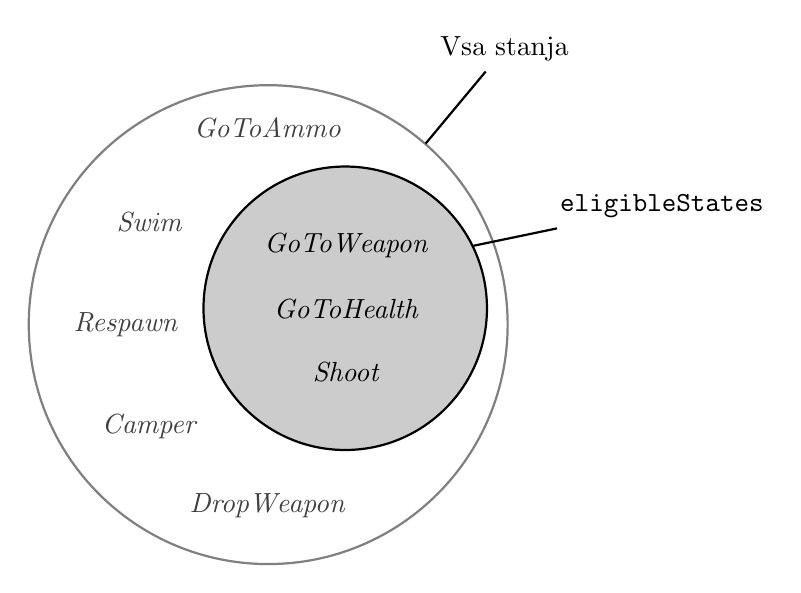
\begin{tikzpicture}[thick]
    % zunanji krog
    \coordinate [] (C) at (2.0,2.3);
    \node [draw,gray, circle through=(C)] at (0:0) {};      
    
    % labela in povezava
    \draw (3,3.5) node(c) {Vsa stanja};
    \draw (C) -- (c);

    % notranji krog
    \coordinate [] (A) at (2.6,1);
    \filldraw[black,fill opacity=0.2] (12:1cm) circle (18mm);      
    
    % labela in povezava
    \draw (5,1.5) node(a) {\texttt{eligibleStates}};    
    \draw (A) -- (a);

    % stanja
    \draw (1cm,1cm) node {\textit{GoToWeapon}};
    \draw (1cm,0.2) node {\textit{GoToHealth}};
    \draw (1,-0.6) node {\textit{Shoot}};
    \draw [darkgray] (0,2.5) node {\textit{GoToAmmo}};
    \draw [darkgray] (-1.5,1.3) node {\textit{Swim}};
    \draw [darkgray] (-1.8,0) node {\textit{Respawn}};
    \draw [darkgray] (-1.5,-1.3) node {\textit{Camper}};
    \draw [darkgray] (0,-2.3) node(b) {\textit{DropWeapon}};
  \end{tikzpicture}
  \caption{Seznam ustreznih stanj v trenutku odločanja, med katerimi izbira arbiter stanj}
  \label{fig:eligible-set-example}
\end{figure}

\section{Nagrajevalno učenje} \label{sec:nagrajevalno-ucenje}
% aka. Reinforcement Learning
\subsection{Splošno o nagrajevalnem učenju}
Ideja, ki se nam je zdela zanimiva je, da se naši agenti na najvišjem nivoji ne bi odločali glede na v naprej zakljenjena pravila, ampak, da bi se vsak agent znal
na podlagi izkušenj naučiti katere akcije so primerne v danem trenutku in katere ne. 

Za realizacijo naše ideje nam je mentor predlagal uporabo metode \textit{nagrajevalnega učenja}\footnote{Reinforcement Learning}. Bistvo te metode je, da se 
agent poskuša z raziskovanjem naučiti kako mora izvajati akcije v svojem okolju, da bo na dolgi rok čimbolje nagrajen.

Prednost uporabe nagrajevalnega učenja, pred npr. nadzorovanim učenjem, je v tem, da nam pri tej metodi ni potrebno eksplicitno specificirati katera akcija
je pravilna za dano stanje - tega se agent nauči z raziskovanjem in preko dobljenih nagrad. Druga prednost je fleksibilen učni postopek, saj lahko brez težav prehajamo med raziskovanjem 
(med katerim se agent uči) in med uporabo dobljenega znanja.

Naloga algoritma za nagrajevalno učenje je, da bo vsota nagrad, ki jih agent dobi z izvajanjem svojih akcije na dolgi rok čimvečja; iščemo torej primerno
\textit{politiko} po kateri se bo ravnal agent. 

\subsection{Q-learning}
Algoritmov s katerimi lahko dosežemo (aproksimacijo) optimalne politike je veliko. V našem primeru vsak agent
uporablja pristop imenovan \textit{Q-learning}\cite{rl}. Prednosti, ki smo jih videli v tem pristopu so:
\begin{itemize}
 \item za ocenjevanje tega kako dobro se bo posamezna akcija obnesla ne potrebujemo modela okolja,
 \item enostavna implementacija in
 \item možnost nadgraditve v SARSA pristop.
\end{itemize}
Okolje s katerim naš agent interaktira je zelo kompleksno (v primerjavi npr. z igro backgammon, ki je pogosto omenjena domena za uporabo nagrajevalnega učenja),
zato se nam je zdel takšen pristop brez modeliranja okolja še posebej privlačen. Pri implementaciji in razumevanju tega principa nam je bil še posebej v pomoč 
vir \cite{rl}.\\\\
Q-learning sloni na podatkovni strukturi, ki za dani par $(stanje, akcija)$ pove vrednost te odločitve (imenovane tudi \textit{Q-value}):
$$Q: S\times A \rightarrow \mathbb{R}$$
Skozi postopek učenja se te vrednosti iterativno popravlja na podlagi dobljene nagrade, stare Q-vrednosti in najvišje možne Q-vrednosti, ki lahko sledi po tej 
akciji (glej \cite{ql}).\\
Čez čas te vrednosti konvergirajo. Če takrat za dano stanje $s$ vedno izberemo tisto akcijo $a$, ki ima največjo Q-vrednost $Q(s, a)$, potem bo agent sledil
optimalni politiki.

\subsection{Integracija v Hivemind}
Problem nagrajevalnega učenja je formuliran kot Markovski odločitveni problem\footnote{Markov decision process ali MDP}. To pomeni, da model nagrajevalnega učenja
predstavimo z
\begin{itemize}
 \item množico stanj,
 \item množico akcij ter
 \item množico realnih števil, ki predstavlja možne nagrade agentu.
\end{itemize}
V našem primeru smo se odločili za naslednjo predstavitev problema. Agent je predstavljen z:
\begin{itemize}
 \item množico stanj, kjer vsako stanje predstavlja agentovo \textit{notranje} ("mentalno") stanje,
 \item množico akcij, ki je v resnici podmnožica \textit{fizičnih} stanj (v prostoru igre), ki jih lahko zavzame agent (npr. stanje Shoot; glej poglavje \textit{Stanja agenta}) in
 \item funkcijo nagrade, ki nagradi akcije, ki so v prid agentu.
\end{itemize}
Odločanje o nadaljnih potezah je abstrahirano v razredu \verb+Brains+, ki je v Hivemind sistem integriran tako, da je povsem transparenten od dejanskih izbranih 
stanj, akcij in nagrad agenta - lahko bi se poigrali in definirali več različic možganov - odvisno od obnašanja, ki bi ga želeli od agenta 
(lahko bi bil agresiven do nasprotnikov, lahko bi bil bolj previden in bi se neprestano zdravil in iskal boljša orožja ipd). Zaradi pomanjkanja časa imamo 
tako le eno različico možgan. Delovanje teh pa podrobneje razložijo naslednja podpoglavja.

\subsubsection{Notranja stanja agenta}
Problem pri nagrajevalnemu učenju lahko nastopi pri prevelikem številu možnih stanj agenta. Takrat lahko postane prostor, ki ga agent raziskuje 
(pri učenju naključno) enostavno prevelik, da bi v doglednem času prišli do optimalne politike obnašanja. Da bi se temu izognili smo morali nekatere 
komponente, ki predstavljajo notranje stanje agenta diskretizirati.\\
Odločili smo se za naslednjo strukturo stanja našega agenta (vsako stanje je vektor, ki lahko zavzame navedene vrednosti):
$$(health \in \{low, mid, high\}, weapon \in \{blaster, shotgun, \ldots\}, ammo \in \{low, high\}, enemyVisible \in \{true, false\})$$
Informacije o tem kakšne so vrednosti komponent možgani dobijo preko posodobitev, ki jih o igralcu pošlje Quake II strežnik in zato niso
nič bolj napredne kot bi jih imel pri igranju človek. Kot smo že omenili, smo želeli, da naši agenti ne goljufajo kot je to običajno pri računalniško
gnanih igralcih pri takih igrah - ponavadi imajo na voljo precej več informacij o svetu kot pa človek.

\subsubsection{Množica akcij}
Agent lahko na okolje vpliva preko množice akcij. Omenili smo že, da je vsaka taka akcija predstavljena s fizičnim stanjem agenta (poglavje \textit{Stanja agenta}),
ki govori o tem kako naj se v vsakem trenutku agent obnaša v svetu.\\
Značilnosti okolja kot ga vidi naš agent je, da je zelo kompleksno in posledično so kompleksne tudi akcije s katerimi agent lahko vpliva na svet - akcije trajajo 
določen čas, agent se lahko med tem fizično premakne, pade v vodo, sreča sovražnika, ipd. Zaradi tega smo se odločili, da akcije modeliramo kot stanja, ki se v 
nekem trenutku zaključijo. \\
Primer: možgani se odločijo naj agent izvede akcijo Shoot. Agent bo šel v fizično stanje Shoot in začel streljati najbližjega sovražnika. Ko sovražnika ne bo 
več ali pa ko sam umre, se bo stanje označilo kot končano. V tem primeru možgani vedo, da se je akcija končala in oceni kako je bila uspešna ter posodobi 
Q-vrednost za dani par $(stanje, akcija)$.\\
Možne akcije, ki jih lahko izvaja agent so:
$$A = \{wander, shootAt, findAmmo, findBetterWeapon, findUpgrade\}$$
Na tem mestu je potrebno omeniti, da se v svetu v katerem so naši agenti ni smiselno ``učiti'' vseh akcij. Za določene akcije lahko rečemo, da so take, da jih
agent izvede kot \textit{refleks}. Primer take akcije oz. fizičnega stanja je iti v stanje plavanja, ko agent pade v vodo, saj je ta akcija ob taki situaciji 
edina smiselna in se prehod v to stanje zgodi brez posredovanja možganov.\\
Omenili smo že, da s številom možnih akcij in stanj narašča prostor, ki ga mora potencialno raziskati agent. Modifikacija, ki smo jo lahko uvedli v našem okolju
je že omenjen seznam \verb+eligibleStates+, ki pove katera stanja so sploh na voljo v danem momentu. To pomeni, da bodo možgani v nekem trenutku imeli
na voljo le akcije (oz. fizična stanja), ki so sploh možne. S tem seveda onemogočimo nesmiselno raziskovanje, ki bi lahko sledilo v nasprotnem primeru.

\subsubsection{Funkcija nagrade}
Postopka po katerem bi dobili uspešno funkcijo nagrade ni. Vprašati se je bilo potrebno po cilju h kateremu bo vsak agent stremel. Agenti skupaj v skupini
tekmujejo proti drugi skupini agentov in zmagovalna bo tista ekipa, ki bo prva dosegla določeno število pobojev nasprotnikov.\\
Pri nagrajevalnem učenju seveda ne moremo eksplicitno govoriti o pravilnih akcijah, ampak le posredno preko nagrad. Odločili smo se, da je agent nagrajen v 
treh primerih:
\begin{itemize}
 \item ko se mu zviša nivo zdravja (nagrada velikosti 1),
 \item ko pobere naboje (nagrada velikosti 1),
 \item ko ubije kakega sovražnika (nagrada velikosti 5).
\end{itemize}
Predpostavljali smo, da če agent stremi po akcijah, ki mu prinašajo zgornje nagrade, potem bo deloval skladno s skupnim ciljem ekipe.

\subsection{Implementacija}
Najbolj običajna implementacija Q-learning postopka je preko \textit{look-up} tabele v kateri se hranijo Q-vrednosti. Taka podatkovna struktura pa 
postane težavna, če imamo veliko množico stanj. V našem primeru to ni bilo težavno, saj je bilo kombinacij stanj sorazmerno malo, lahko pa bi bilo
problematično, če nekaterih vrednosti ne bi diskretizirali.\\
Alternativna možnost za implementacijo pa je z uporabo prilagojene umetne nevronske mreže \cite{ql}. V tem primeru nevronska mreža vrača kar
Q-vrednosti. To pa predstavlja tudi možnost za nadaljne delo - preskusiti kako bi se obneslo nagrajevalno učenje skupaj z nevronsko mrežo, saj
v tem primeru diskretizacija komponent vektorja stanja agenta morda ne bi bila potrebna in zanimivo bi bilo videti kakšna bi bila v tem primeru
videti optimalna politika obnašanja.\\
V sklopu našega projekta se Q-vrednosti hranijo v \textit{look-up} tabeli. Taka tabela je abstrahirana v posebno podatkovno strukturo, ki na podlagi dejstva, 
da imamo končno število stanj in akcij, oštevilči vsak tak vektor (ali stanja ali akcije, če bi akcija imela več komponent) in tako na podlagi te enolične 
identifikacije dostopa do Q-vrednosti, ki jo hrani za tak par $(stanje, akcija)$.

\subsection{Obstojnost znanja}
V sistemu, ki smo ga razvili lahko ob zagonu z zastavico povemo ali naj se v tej seji agent uči oz. ali naj uporablja že pridobljeno znanje (specificirano
z datoteko). 
Če se agent uči, potem na določene časovne intervale shranjujemo vso znanje (Q-vrednosti), ki jih je agent pridobil do tega trenutka, v datoteko. Tako datoteko lahko potem
agent v naslednjih sejah spet uvozi in jo uporablja naprej.

\section{Komunikacija med agenti}

Ogrodje omogoča tudi komunikacijo med večimi agenti, ki predstavljajo skupino. Ta komunikacija omogoča, da nekatere naloge opravijo veliko hitreje kot sicer (npr. že omenjeno raziskovanje sveta in generiranje topografije) in tudi da lahko sodelujejo pri določenih akcijah.

\subsection{MOLD (Message Oriented Lightweight Distributor)}

Na začetku nam je bilo priporočeno ogrodje CAST\footnote{CoSY Architecture Schema Toolkit}, ki je namenjeno prav skupinski komunikaciji različnih agentov oz. lahko tudi delov agentov. Uporablja paradigmo \textit{skupne table}, na katero različni agenti dodajajo svoje znanje o problemu, ki naj bi ga trenutno reševali. Pisanje na tablo je v osnovi predstavljeno kot sporočilo, ki ga nek agent pošlje vsem ostalim, prejmejo pa ga vsi, ki so se na tak tip sporočila naročili.

To se mogoče zdi v redu, vendar je sama implementacija CAST-a in njegov pristop popolnoma prekompleksen in nepotreben za dano situacijo. Pri raziskovanju le-tega smo naleteli na naslednje probleme:
\begin{enumerate}
  \item Neverjetno pomanjkanje dokumentacije ter predvsem opisa notranjega delovanja ogrodja. Manjkajo relacije med posameznimi deli in podroben opis postopka serializacije ter hranjenja sporočil.
  
  \item Za serializacijo se uporablja neka pretirano obsežna knjižnica imenovana ICE, ki je sama po sebi skoraj tako velika kot CAST. Prav tako ICE hkrati rešuje dva problema, serializacijo in komunikacijo, kar naredi rešitev nefleksibilno za takšno preprosto uporabo kot je naš sistem.
  
  \item Ogrodje želi poleg problema same komunikacije (nespametno) reševati tudi problem postavitve (\textit{deployment}). Na tak način se programu ne predstavlja kot knjižnica, temveč želi postati kar vstopna točka (\textit{entry point}) za izvajanje celotnega programa. To komplicira sistem prevajanja in tudi onemogoča fleksibilnost rešitve.
\end{enumerate}

Zaradi teh razlogov smo se odločili, da bo lažje v kolikor implementiramo svoj lasten protokol komunikacije. Imenovali smo ga MOLD, temelji pa na nekaj precej enostavnih principih.

\subsubsection{Topologija}

Osrednja ideja MOLD-a je zastavljena kot podatkovno vodilo. Posamezni agenti se na vodilo povežejo, na njem nastopajo s svojimi unikatnimi identifikatorji, ter med sabo s pomočjo vodila komunicirajo. Samo vodilo ne ponuja nobene druge storitve razen prenašanja ustrezno formatiranih sporočil med agenti, vsa komunikacija pa poteka preko TCP/IP povezav. Katerikoli agent lahko neodvisno od drugih kadarkoli na vodilo pošlje sporočilo, naloga vodila je torej zgolj to da to sporočilo dostavi naslovniku (eden ali cela skupina agentov).

\subsubsection{Serializacijski format}

Vsak fleksibilen protokol potrebuje tudi fleksibilen in učinkovit serializacijski format, ki se bo prenašal neposredno preko TCP/IP povezave. Takšna odlična knjižnica razvita prav v ta namen je Googlova knjižnica Protocol Buffers. Zelo dobra lastnost je to, da je \texttt{protobuf} namenjena zgolj serializaciji in ne poskuša implementirati tudi drugih stvari mrežne komunikacije (za razliko od ICE-a in CAST-a). Nadaljnji primeri sporočil bodo zapisani v \texttt{protobuf} notaciji, zato priporočamo, da se bralec z njo na tem mestu seznani.

\subsubsection{Sporočila}

Celoten protokol komunikacije med našimi agenti sestoji iz sporočil. Ta sporočila so brez stanja (za razliko od CAST-a, kjer trenutno stanje predstavlja sama tabla) in so lahko namenjena celotni skupini ali pa zgolj določenemu posameznemu agentu. Vsako sporočilo je predstavljeno v naslednji obliki:

\begin{verbatim}
message Message {
  // Valid packet types
  enum PacketType {
    CONTROL_ANNOUNCE = 1;
    EVENT_LOCATION_UPDATE = 2;
    EVENT_RESPAWNED = 3;
    EVENT_ENTITY_UPDATE = 4;
    // ...
  };
  
  // Source/dest bot identifiers
  required string sourceId = 1;
  optional string destinationId = 2;
  
  // Timestamp
  required uint64 timestamp = 3;
  
  // Type
  required PacketType type = 4;
  
  // Payload
  required bytes data = 5;
};
\end{verbatim}

\noindent
To je osnovna ovojnica vsakega sporočila in takšna sporočila se prenašajo preko MOLD vodila. Glede na tip sporočila ima lahko vsako tako sporočilo še dodatno vsebino, ki se nahaja v \texttt{data} bloku. Vodilo vidi samo ta prvi nivo sporočila, kar omogoča učinkovito in hitro posredovanje sporočil med agenti (vmesna deserializacija ni potrebna). Za samo izvedbo komunikacije se ne uporablja večnitnosti, temveč asinhron način komunikacije, kjer vse vhodno/izhodne operacije ne blokirajo programa. Vse to poskrbi za maksimalno pretočnost vodila.

\subsection{Potek komunikacije}

Kot že rečeno si agenti med sabo izmenjujejo sporočila. Za izmenjevanje sporočil z drugimi agenti je odgovoren komunikacijski podsistem ogrodja. Le temu podsistemu je dovoljeno, da neposredno sprejema in pošilja MOLD sporočila. Na tak način je pretok sporočil in notranjih dogodkov nadzorovan, kar olajša razhroščevanje.

Posamezni deli agenta lahko v vsakem trenutku sprožijo notranje dogodke. Ti dogodki se npr. prožijo v primeru da agent odkrije neko novo entiteto ali pa npr. umre. Takšni notranji dogodki služijo za komunikacijo med posameznimi deli agenta, prav tako pa jih prestreže komunikacijski podsistem, da o dogajanjih obvešča tudi druge agente. Le-ta je odgovoren tudi za procesiranje prispelih sporočil ter morebitnemu proženju notranjih dogodkov ostalim komponentam.

Nekaj pomembnih sporočil, ki nastopajo v komunikaciji ter njihova uporaba in interakcija z notranjimi komponentami, je opisanih v nadaljevanju.

\subsubsection{Razglas prisotnosti agenta na vodilu}

Ko se agent prvič uspešno poveže na vodilo mora najprej na nek način ugotoviti kdo vse je mogoče še prisoten na vodilu. Ker samo vodilo te storitve ne omogoča, agenti implementirajo razglasni protokol.

Vsak agent takoj ob povezavi na vodilo pošlje sporočilo tipa \texttt{CONTROL\_ANNOUNCE}, ki ima naslednjo obliko:
\begin{verbatim}
message Announcement {
  // Name
  required string name = 1;
  
  // Entity identifier
  required uint32 entityId = 2;
  
  // Reply marker
  required bool reply = 3;
};
\end{verbatim}

\noindent
Vsebuje unikatni naziv agenta, identifikator njegove entitete na Quake II strežniku ter oznako ali gre za odgovor ali ne. Vsak agent, povezan na vodilo, ki prejme takšno sporočilo odgovori s svojim razglasom, le da oznako \texttt{reply} postavi na \texttt{true}. Ta oznaka preprečuje neskončne odgovore na razglase.

Ti razglasi pa pri vsakem od agentov povzročijo dodajanje agenta v lokalni imenik (tega ima vsak agent pri sebi), ki omogoča poizvedbe ali je določena entiteta prijatelj ali sovražnik ter tudi sledenje lokaciji agenta.

\subsubsection{Sporočanje lokacije agenta in potrjevanje prisotnosti}

Lokacijo agenta, ki se prav tako hrani v imeniku, mora vsak agent periodično posodabljati tako da na vodilo pošilja sporočila tipa \texttt{EVENT\_LOCATION\_UPDATE}. V kolikor tega ne stori vsaj vsakih 60 sekund je brisan iz imenika. V resnici agenti svojo lokacijo obnavljajo veliko bolj pogosto (ob vsaki spremembi ali vsakih 500 milisekund, kar pride prej).

Vsako sporočilo preprosto vsebuje koordinate lokacije na kateri se trenutno nahaja agent:
\begin{verbatim}
message LocationUpdate {
  // Coordinates
  required float x = 1;
  required float y = 2;
  required float z = 3;
}
\end{verbatim}

\noindent
Katerikoli agent, ki prejme tako sporočilo posodobi vnos v imeniku v kolikor le-ta že obstaja. V kolikor pa vnosa ni (kar se lahko zgodi v kolikor je agent ravno prispel na vodilo ali pa ker je morebiti ciljni agent zgrešil kakšno sporočilo), izvornemu agentu (in samo njemu) nemudoma pošlje svoj razglas.

Periodično sporočanje lokacije tako služi dvem nalogam, po eni strani omogoča sledenje premikom posameznih agentov (to izkorišča tudi podsistem za navigacijo, da se iz premikov ostalih agentov uči topografije sveta), po drugi strani pa služi kot indikator da je agent še vedno povezan na vodilo (samo vodilo samo po sebi namreč ne omogoča nikakršne evidence o tem kdo je nanj povezan, to informacijo morajo vzdrževati agenti sami).

\subsubsection{Obveščanje agentov o premikih videnih entitet}

Za potrebe celostnega pogleda na svet, se agenti med seboj obveščajo o vseh dinamičnih entitetah, ki jih v svetu vidijo. Pogled vsakega izmed agentov je namreč (s strani virtualnega sveta, torej Quake II strežnika) omejen na njegovo lokalno okolico, skupaj pa imajo tako možnost da pridobijo dodatne informacije, ki jih vsak posamezen agent nima.

Sporočila se pošiljajo zgolj v kolikor se stanje določene vidne entitete na kakršenkoli način spremeni in so naslednje oblike:
\begin{verbatim}
message EntityUpdate {
  // Coordinates
  required float x = 1;
  required float y = 2;
  required float z = 3;
  
  // Entity identifier
  required uint32 entityId = 4;
  
  // Model index
  required uint32 modelIndex = 5;
  
  // Player or not
  required bool player = 6;
}
\end{verbatim}

\noindent
Vsak agent, ki prejme takšna sporočila lahko integrira podatke o entiteti v svojo notranjo predstavitev sveta. Prav tako se ta spročila uporabljajo za hitrejše učenje topografije sveta, saj lahko agenti na tak način sledijo večjemu številu drugih igralcev.

\subsubsection{API za glasovanja}

Velikokrat se lahko zgodi, da se morajo agenti v skupini skupaj odločiti kdo bo nekaj napravil. V ta namen smo v naše ogrodje vključili API, ki naredi takšno glasovanje transparentno. Vsak agent lahko ustvari anketo določene kategorije in zahteva od skupine da zanjo glasujejo. Do glasovanja so upravičeni vsi člani, ki so bili v trenutku začetka znani v agentovem lokalnem imeniku.

Vsaki anketi je dodeljen unikatni identifikator, sporočilo, ki zahteva novo anketo je tipa \texttt{POLL\_CREATE} in ima naslednjo strukturo:
\begin{verbatim}
message PollCreate {
  // Unique poll identifier
  required string pollId = 1;
  
  // Expiry timestamp
  required uint32 closesOn = 2;
  
  // Voting category
  required string category = 3;
}
\end{verbatim}

Vsak agent lahko glasuje v kolikor ima za dano kategorijo registriran \textit{glasovalni modul}. Naloga tega modula je da se na podlagi lokalnih informacij, ki so agentu na voljo, odloči in odda svoj glas. Glasovanje poteka s sporočili tipa \texttt{POLL\_VOTE} z naslednjo strukturo:
\begin{verbatim}
message PollVote {
  // Unique poll identifier
  required string pollId = 1;
  
  // Choice and amount of votes
  required string choice = 2;
  required float votes = 3;
}
\end{verbatim}

Agentje svoje glasove oddajo neposredno tistemu, ki je anketo ustvaril, tako da ne obremenjujejo vodila in ostalih agentov z nepotrebnimi sporočili. Kdor je anketo zahteval je odgovoren tudi za štetje glasov po končanem glasovanju. Glasovanje se samodejno zaključi ko ali glasujejo vsi agenti, ki so do glasovanja upravičeni, ali pa preteče čas, ki je odvisen od dane ankete.

Znotraj posameznega agenta se ob končani anketi generira ustrezen dogodek, ki je na voljo posameznim komponentam agenta.

Trenutno so implementirani naslednji glasovalni moduli:
\begin{itemize}
  \item \texttt{DummyVoter}, ki se uporablja za periodično testiranje delovanja glasovanja kjer agentje glasujejo z naključnimi vrednostmi.
  
  \item \texttt{DroperVoter}, ki glasuje na podlagi tega ali ima agent na voljo kakšno orožje odveč in glede na razdaljo od agenta, ki je zahteval glasovanje. Na tak način se izbere agent, ki bo na novo \textit{respawnanemu} agentu prinesel orožje.
\end{itemize} 

\section{Možne izboljšave}

Med razvojem ogrodja in raziskovanjem področja smo odkrili nekaj možnosti za izboljšave, katerih na žalost zaradi pomanjkanja časa nismo uspeli preveriti.

\begin{itemize}
  \item Implementirati iskalni algoritem, omenjen v \cite{champandard02}, za inkrementalno izboljševanje poti od trenutne pozicije do vseh ostalih točk. Bistvena lastnost algoritma je, da lahko pri gradnji poti upošteva da se na nekaterih vozliščih nahajajo nagrade (različni predmeti) za katere je včasih dobro vzeti malo daljšo pot. Dobra stvar je tudi, da se drevo poti gradi postopoma in upošteva majhne spremembe korena (tako da ni potrebno vsakič zgraditi drevesa popolnoma na novo, kar močno izboljša performanse).
  
  \item Ugotoviti zakaj naš sistem EANN ni konvergiral v doglednem času.
  
  \item Raziskati možnost arhitekture, ki omogoča zlivanje različnih stanj. Na tak način bi agent lahko kombiniral svoje zmožnosti, kar bi mu dodalo veliko večjo fleksibilnost.
  
  \item Raziskati možnost sledenja gladkim potem skozi več točk, ki so generirane s pomočjo Catmull-Romovih zlepkov. Prav tako bi lahko iskanje poti upoštevalo kote med zaporednimi točkami in izbiralo takšne točke, ki minimizirajo zavoje.

  \item Implementacija poizvedb za Q-vrednosti s prilagojeno umetno nevronsko mrežo. V tem primeru je prostor stanj lahko veliko večji, kar bi lahko prineslo
        določene prednosti pri obnašanju agentov.
\end{itemize}

\section{Zaključek}

Vsa izvorna koda je izdana pod licenco GPLv3 in se skupaj z dnevnikom razvoja nahaja na:

\begin{center}
\texttt{http://code.google.com/p/q2hivemind}
\end{center}

%
% Literatura
%
\begin{thebibliography}{9}

\bibitem{champandard02}
  Alex J. Champandard,
  \emph{Realistic Autonomous Navigation in Dynamic Environments}.
  Institute of Perception Action and Behaviour,
  Edinburgh University,
  2002.

\bibitem{seymour08}
  Peter Seymour,
  \emph{Off-the-shelf Genetic Algorithm Optimiser}.
  http://www.bluestretch.com/mendelsolve/offshelf\_ga.ps,
  2008.

\bibitem{grayston06}
  Thomas Ian Grayston,
  \emph{A Simplified Fuzzy-Logic Control System Approach to Obstacle Avoidance combining Stereoscopic Vision and Sonar}.
  School of Computing,
  University of Tasmania,
  2006.

\bibitem{batagelj97}
  Batagelj V., Mrvar A.
  \emph{Pajek - Program for Large Network Analysis}.
  Sunbelt,
  1997.

\bibitem{harris08}
  Paul Harris, Sylvain Bougerel,
  \emph{libkdtree++, C++ kd-tree Library}.
  http://libkdtree.alioth.debian.org/,
  2008.

\bibitem{rl}
  Mark Humphrys,
  \emph{Action Selection methods using Reinforcement Learning},
  PhD thesis, 2. poglavje,
  http://www.compapp.dcu.ie/~humphrys/PhD/index.html

\bibitem{ql}
  Wikipedia,
  \emph{Q-learning},
  http://en.wikipedia.org/wiki/Q\_learning

\end{thebibliography}

\end{document}

